%!TEX root = ../../adrien_gomar_phd.tex

\chapter*{Conclusion}

The industrial design of turbomachinery, and by extension Contra-Rotating
Open Rotors (CROR), is usually based on steady flow analysis. 
However, this approach finds its limits 
when unsteady phenomena become dominant. This is the case of 
CROR where the interaction between the
two rotors is of prior importance. In such a
context, engineers need now tools to account for these effects as
early as possible in the design cycle. With the growth of
computational power, unsteady computations are entering industrial
practice, but the associated restitution time remains an obstacle for
daily basis applications. For this reason, efficient
unsteady approaches are receiving a lot of attention. 

Fourier-based methods for periodic flows have undergone major
developments in the last decade (see \citet{He2010} for a recent
review). The basic idea is to decompose
time-dependent flow variables into Fourier series, which are then
injected into the equations of the problem. The time-domain problem is
thus made equivalent to a frequency-domain problem, where the complex
Fourier coefficients are the new unknowns.
At this point, two
strategies coexist to obtain the solution. The first one is to solve
directly the Fourier coefficients, using a dedicated
frequency-domain solver, as proposed by \citet{He1998}. 
The second strategy is to cast the
problem back to the time domain using the inverse Fourier transform, as
proposed by \citet{Hall2002} with the Harmonic
Balance (HB) method. The unsteady time-marching problem is thus
transformed into a set of steady equations coupled by a source term.
This last is a high-order spectral evaluation of the time-derivative of the
initial equations. The main advantage of solving in the time domain is
that it can be implemented in an existing classical RANS solver,
taking advantage of all classical convergence-accelerating techniques
for steady state problems.

Recently, \citet{ThesisGuedeney} developed and implemented a
multi-frequential HB method into the \emph{elsA} CFD solver. 
This method allows to compute unsteadinesses whose frequencies
are not harmonically related, which opens new perspectives
such as CROR aeroelasticity.
In this framework, the goal of this study 
was to assess the multi-frequential 
harmonic balance applied to the aeroelasticity of CROR. 

\section*{Summary of the results}

\subsection*{On the conditioning of multi-frequential harmonic balance methods}

When unsteadiness is related to a single frequency and its
harmonics, Fourier analysis leads to a natural choice for time instances
needed to compute the source term:
they are evenly spaced over the period. In this case, the mathematical
problem is numerically well-defined, meaning that the conditioning of
the operators ensures the convergence of the approach.
In opposite, when several arbitrary frequencies are 
considered, as for instance CROR
aeroelasticity, the multi-frequential harmonic balance approach
is required but its source term can be ill-conditioned.

In \hyperref[cha:limitations_condition_number]{\emph{Chapter~5}},
we demonstrated that the time sampling has a major effect on the
stability of the multi-frequential harmonic balance 
method, due to the condition number of the Fourier
transform matrix. One way to tackle this issue, 
is to consider a non-uniform time sampling
along with an algorithm to properly choose the time instances
as proposed by \citet{ThesisGuedeney}.
The Almost-Periodic Fourier Transform algorithm (APFT) 
algorithm, originally developed by \citet{Kundert1988} and implemented by 
\citet{ThesisGuedeney}, is shown to improve the
Fourier matrix orthogonality and thus the condition number.
However, for segregated frequencies, the condition number
remains too large to be used within an industrial context.

As the aeroelasticity of CROR is by essence
composed of segregated frequencies, new algorithms are needed.
This is why, a gradient-based OPTimization algorithm (OPT) 
has been developed in the current work.
It directly minimizes the condition number thanks to a
gradient-based optimization method. This last has proved to
give a condition number that is almost unity for any input frequencies,
thus alleviating the stability issues encountered for HB
computations composed of segregated frequencies.
Therefore, the non-uniform time sampling proposed by \citet{ThesisGuedeney}
used together with the OPT algorithm 
developed in the present contribution
enables to tackle problems with large frequency 
separation or large unsteadinesses, namely CROR aeroelasticity
can be considered.
This work has been published in:
\begin{quote}
	{\small T. Gu\'edeney, \emph{A. Gomar}, F. Gallard, F. Sicot, G. Dufour, and G. Puigt. 
	Non-Uniform Time Sampling for Multiple-Frequency Harmonic Balance Computations. 
	\emph{Journal of Computational Physics}, 236:317--345, March 2013}
\end{quote}


\subsection*{On the convergence of Fourier-based time methods}

Efficiency of Fourier-based time methods results 
from a trade-off between accuracy and 
costs requirements.
On one hand, the accuracy depends on the number of harmonics
used to represent the frequency content of the time 
signal; on the other hand, computational costs and 
memory consumption of the computations also scale
with the number of harmonics. 
The problem is that this number of harmonics is 
configuration-dependent and hardly predictable. 
Moreover, a high number of harmonics
($\gg 10$) can prevent the use of such an approach,
as it might be more expansive than the classical time-marching approaches.
This is particularly true on CROR configurations were the number
of harmonics needed have been shown to be greater than ten
on some configurations.

In \hyperref[cha:limitations_convergence]{\emph{Chapter~6}}
we investigated the accuracy and convergence properties 
of Fourier-based time integration methods, among which the
HB approach used in this work. It is shown that the convergence rate 
of these methods, in terms of harmonics required to describe the solution 
with a given level of accuracy, depends on the spectral content of the 
solution itself: Fourier-based time methods are particularly efficient 
for flow problems characterized by a narrow Fourier 
spectrum. 

We showed that the main source of unsteadiness in 
turbomachinery flows is due to the relative motion of wakes 
generated by a given blade row with respect to the downstream row.
Statistically speaking, the passing wakes are seen by the downstream 
row as an azimuthally advected periodic Gaussian pulse, 
characterized by its relative thickness
and by the velocity deficit associated to it.
The Fourier transform of a Gaussian function being analytical,
an truncation error has been defined, which showed that the narrower the wake, 
the larger its Fourier spectrum resulting in a slower convergence 
of Fourier-based time methods.

Based on this knowledge of the phenomenon,
we showed on a model turbomachinery computation, that
the analytical truncation error can be \emph{a priori} 
estimated using a mixing-plane steady computation
using the azimuthal accumulated energy.
We showed that a 10\% error (or equivalently 
a 99\% accumulation of energy) is a good threshold
that ensures the continuity of the wakes at the rows
interfaces, which was the motivation of the current study.
Applying the \emph{a priori} error estimate to 
the steady computation of any turbomachinery configuration
gives the number of harmonics required to ensure the
convergence of the Fourier-based time method.

This preliminary step has a negligible cost compared to the overall 
simulation, since the steady computation is classically used to initialize 
the unsteady run, and extraction of wake characteristics takes 
less than a minute on a single processor. 
This work has been submitted in:
\begin{quote}
	{\small \emph{A. Gomar}, Q. Bouvy, F. Sicot, G. Dufour, P. Cinnella, and B. Fran\c cois. Convergence of Fourier-based time methods for turbomachinery wake passing problems. 
	\emph{Journal of Computational Physics}, submitted in December 2013}
\end{quote}

The prediction tool

\subsection*{On the aeroelasticity of contra-rotating open rotors}

In \hyperref[cha:stcf11]{\emph{Chapter~7}}, 
the proposed weak coupling approach along with
an harmonic balance approach has been
validated on the $11^{th}$ standard aeroelastic turbomachinery
configuration.
The results show that the harmonic balance approach provides local
and global results close to the reference time-marching scheme 
with only $N=1$ harmonic in the time period. At the cost of a memory
increase (roughly equal to the number of instances used in the harmonic balance
simulations), the computational saving is seven for this
particular case compared to a phase-lag approach combined
with a time-marching scheme. Moreover, the results are
in good agreement with the experimental data and with the results
found in the literature, validating the current approach.






\section*{Future work}

\begin{figure}[htp]
  \centering
  \subfigure[2F]{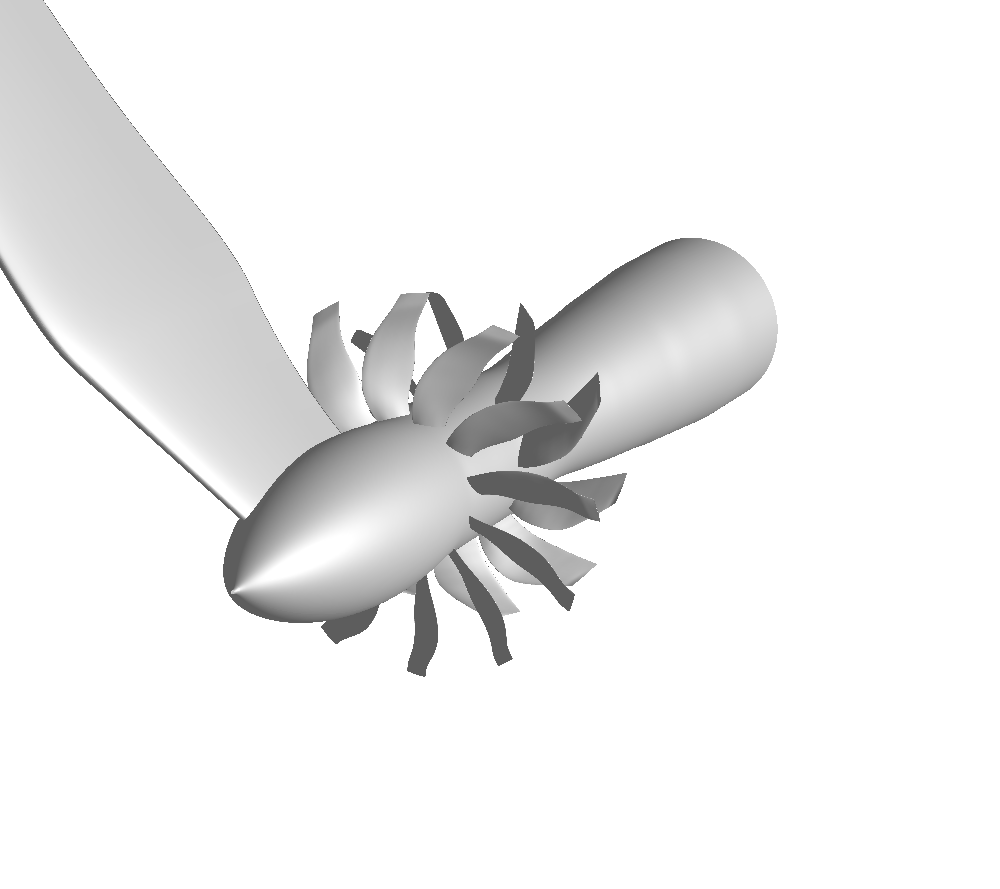
\includegraphics[width=.4\textwidth]{HERA3_INSTALLED_wall.png}}
  \subfigure[1T]{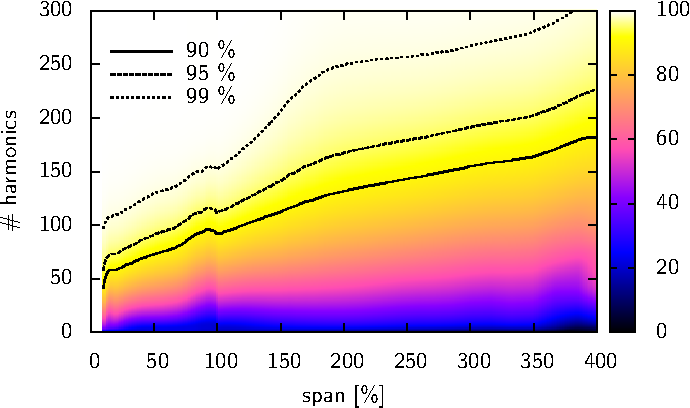
\includegraphics[width=0.40\textwidth]{HERA3_INSTALLED_RANS_SPECTRUM_PPT.pdf}}
  \caption{Low-speed isolated configuration: structural modes considered.}
  \label{fig:hera3_perspectives}
\end{figure}
